% (The MIT License)
%
% Copyright (c) 2022-2025 Yegor Bugayenko
%
% Permission is hereby granted, free of charge, to any person obtaining a copy
% of this software and associated documentation files (the 'Software'), to deal
% in the Software without restriction, including without limitation the rights
% to use, copy, modify, merge, publish, distribute, sublicense, and/or sell
% copies of the Software, and to permit persons to whom the Software is
% furnished to do so, subject to the following conditions:
%
% The above copyright notice and this permission notice shall be included in all
% copies or substantial portions of the Software.
%
% THE SOFTWARE IS PROVIDED 'AS IS', WITHOUT WARRANTY OF ANY KIND, EXPRESS OR
% IMPLIED, INCLUDING BUT NOT LIMITED TO THE WARRANTIES OF MERCHANTABILITY,
% FITNESS FOR A PARTICULAR PURPOSE AND NONINFRINGEMENT. IN NO EVENT SHALL THE
% AUTHORS OR COPYRIGHT HOLDERS BE LIABLE FOR ANY CLAIM, DAMAGES OR OTHER
% LIABILITY, WHETHER IN AN ACTION OF CONTRACT, TORT OR OTHERWISE, ARISING FROM,
% OUT OF OR IN CONNECTION WITH THE SOFTWARE OR THE USE OR OTHER DEALINGS IN THE
% SOFTWARE.

\documentclass{article}
\usepackage{../ppa}
\newcommand*\thetitle{Abstract Machines}
\newcommand*\thesubtitle{Turing, LLVM, Lambda, SECD, Semantics}
\begin{document}

\lnTitlePage{5}{10}{IPbuj67q5NM}

\pptToc

\plush{\pptChapter[Machines]{Who Are Abstract Machines?}}

\pptSection{Definition}

An \emph{abstract machine} is a theoretical \emph{model} of computation.

Similar to a function, a machine receives \emph{inputs} and produces \emph{outputs} based on predefined \emph{rules}.

Abstract machines are ``machines'' because they allow \emph{step-by-step} execution of programmes. (really?)

They are ``abstract'' because they ignore many aspects of actual (hardware) machines.

An abstract machine is an \emph{intermediate language} with a small-step operational semantics.

\plush{}

\pptSection{Purpose}

``The implementation of a programming language consists of two
stages. The implementation of the compiler and the implementation of the abstract (virtual?) machine.
This is a typical divide-and-conquer approach.
From a pedagogical point of view, this simplifies the presentation and
teaching of the principles of programming language implementations.
From a software engineering point of view, the introduction of layers of
abstraction increases maintainability and portability.'' (\href{https://www.sciencedirect.com/science/article/abs/pii/S0167739X99000886}{1999})

We are interested in using abstract machines to explain the \emph{semantic} of a program.

\plush{}

\pptSection{Virtual Machines}

An abstract machine implemented in software is termed a \emph{virtual machine},
and one implemented in hardware is called simply a ``machine.''

JVM (for Java) and CLR (for .NET) are among most notable examples of virtual machines.

IR (\emph{intermediate representation}) is used internally by a compiler or virtual machine to represent source code.
An \emph{intermediate language} is the language of an abstract machine.

\plush{}

\pptSection{LLVM}

LLVM (Low Level Virtual Machine) is a standard de-facto.

\pptPic{0.7}{llvm.png}

\plush{}

\plush{\pptChapter[Turing]{Turing Machine}}

Turing Machine was the first (1936) ... but not the simplest.

\pptPic{0.7}{turing.png}

For example, Emil Post's Machine is simpler.

\plush{}

\pptSection{Proof}

The \emph{Church-Turing thesis}: Anything that can be computed can be computed by some Turing machine.

There \textbf{has never been a proof}, but the evidence for its validity comes from the fact that every realistic model of computation, yet discovered, has been shown to be equivalent. --- \href{https://mathworld.wolfram.com/Church-TuringThesis.html}{here}.

\plush{}

\plush{\pptChapter[$\lambda$]{$\lambda$-calculus}}

Abstraction:
\begin{equation*}
(\lambda x . t)\quad\quad \text{e.g.}\; f = \lambda x . \sqrt{x}
\end{equation*}

Application:
\begin{equation*}
(t s)\quad\quad \text{e.g.}\; (f\;16) = 4
\end{equation*}

In lambda calculus, \emph{functions} are taken to be ``first class values,''
so functions may be used as the inputs, or be returned as outputs from other functions.

\plush{}

\plush{\pptChapter[SECD]{SECD Machine(s)}}

There are SECD (\textbf{s}tack, \textbf{e}nvironment, \textbf{c}ontrol, \textbf{d}ump),
CESK, CEK, CS, and maybe other abstract machines.

I like the CRM (\textbf{c}ontrol stack, \textbf{r}esult stack, \textbf{m}emory) machine explained by
\href{https://software-lab.org/people/Michael_Pradel.html}{Michael Pradel} in
\href{https://www.youtube.com/watch?v=YRfb2zDk_qs}{his YouTube course} about program analysis:
$\langle c, r, m\rangle$.

\begin{equation*}
\begin{split}
\langle \texttt{x} \mathrel{\texttt{:=}} 2 \times 3, \texttt{nil}, \{\} \rangle
  & \longrightarrow \langle \texttt{x} \mathrel{\circ} 2 \times 3 \mathrel{\circ} \mathrel{\texttt{:=}}, \texttt{nil}, \{ \}\rangle \\
  & \longrightarrow \langle 2 \times 3 \mathrel{\circ} \mathrel{\texttt{:=}}, \texttt{x} \mathrel{\circ} \texttt{nil}, \{ \}\rangle \\
  & \longrightarrow \langle \mathrel{\texttt{:=}}, \texttt{6} \mathrel{\circ} \texttt{x} \mathrel{\circ} \texttt{nil}, \{ \}\rangle \\
  & \longrightarrow \langle \texttt{nil}, \texttt{nil}, \{ \texttt{x} \mapsto 6 \}\rangle \\
\end{split}
\end{equation*}

\plush{}

\plush{\pptChapter{Semantic}}

This is our programming language that helps us draw on a canvas:

\begin{multicols}{2}
{\ttfamily
L 10, 20, 15, 23; \\
C 13, 13, 35; \\
L 5, 28, 15, 12;}

Its semantic may be explained by the abstract machine with the following instruction set, which semantic is \textbf{obvious} to a reader:
\par\columnbreak\par

\begin{tikzpicture}[scale=3,line width=4pt]
\path[draw] (1, 2) -- (1.5, 2.3);
\path[draw] (.5, 2.8) -- (1.5, 1.2);
\node[circle,minimum height=3.5cm,draw] at (1.3, 1.3) {};
\end{tikzpicture}
\end{multicols}

{\ttfamily DRAW x, y; \\
LOOP; IF t THEN BREAK; END LOOP; \\
x > y; x + y; x - y; x / y; \\
x := y; \\
1600; 900.}

\plush{}

This is what "\texttt{L x1, y1, x2, y2}" means:

\begin{multicols}{2}
{\ttfamily
dx := x2 - x1;\\
dx := dx / 1600;\\
dy := y2 - y1;\\
dy := dy / 900;\\
LOOP;\\
DRAW x1, y1;\\
IF x1 > x2 THEN BREAK;\\
IF y1 > y2 THEN BREAK;\\
x1 := x1 + dx;\\
y1 := y1 + dy;\\
END LOOP;}
\par\columnbreak\par
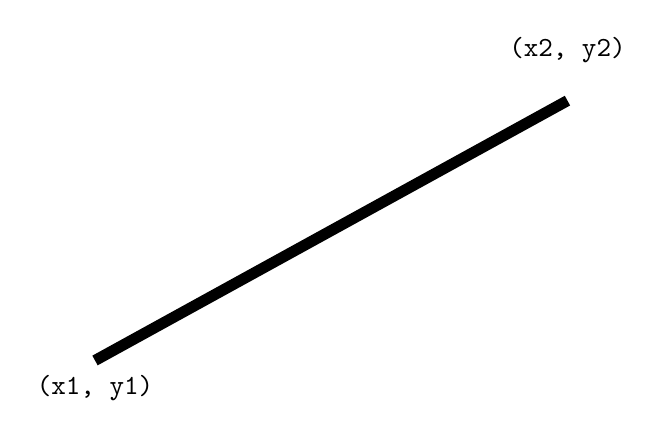
\begin{tikzpicture}[scale=3,line width=4pt]
\path[draw] (.5, .7) -- (2.5, 1.8);
\node[anchor=north] at (.5, .7) {\texttt{(x1, y1)}};
\node[anchor=south] at (2.5, 1.9) {\texttt{(x2, y2)}};
\end{tikzpicture}
\end{multicols}

\end{document}
